\documentclass[a4paper,12pt]{article}
\usepackage[brazil, english]{babel}
\usepackage[utf8]{inputenc}
\usepackage[T1]{fontenc}
\usepackage{geometry}
\usepackage{setspace}
\usepackage{titlesec}
\usepackage{hyperref}
\usepackage{graphicx}
\usepackage{caption}
\usepackage{subcaption}
\usepackage{fancyhdr}
\setlength{\headheight}{15pt}
\addtolength{\topmargin}{-2.5pt}
\usepackage{xcolor}
\usepackage{amsmath, amssymb, bm}
\usepackage{mathtools}
\usepackage{cancel}
\usepackage{tikz}
\usepackage{newunicodechar}
\usepackage{ragged2e}
\usepackage{setspace}
\usepackage{tikz-3dplot} % Necessário para coordenadas 3D
\usetikzlibrary{intersections}
\usepackage{siunitx}
\usetikzlibrary{3d, arrows.meta}
\usepackage{booktabs}


\usepackage{color}
\definecolor{myblue}{rgb}{.8, .8, 1}

\definecolor{ao(english)}{rgb}{0.0, 0.5, 0.0}

\usepackage{amsmath}
\usepackage{empheq}

\newlength\mytemplen
\newsavebox\mytempbox

\makeatletter
\newcommand\mybluebox{%
    \@ifnextchar[%]
       {\@mybluebox}%
       {\@mybluebox[0pt]}}

\def\@mybluebox[#1]{%
    \@ifnextchar[%]
       {\@@mybluebox[#1]}%
       {\@@mybluebox[#1][0pt]}}

\def\@@mybluebox[#1][#2]#3{
    \sbox\mytempbox{#3}%
    \mytemplen\ht\mytempbox
    \advance\mytemplen #1\relax
    \ht\mytempbox\mytemplen
    \mytemplen\dp\mytempbox
    \advance\mytemplen #2\relax
    \dp\mytempbox\mytemplen
    \colorbox{myblue}{\hspace{1em}\usebox{\mytempbox}\hspace{1em}}}
\makeatother

\usepackage[most]{tcolorbox}

\newtcbox{\mymath}[1][]{%
    nobeforeafter, math upper, tcbox raise base,
    enhanced, colframe=blue!30!black,
    colback=blue!30, boxrule=1pt,
    #1}

\tcbset{
    highlight math style={
        enhanced,
        colframe=red!60!black,
        colback=yellow!50,
        arc=4pt,
        boxrule=1pt,
        drop fuzzy shadow
    }
    }

\usepackage{physics}
\usepackage{pgfplots}
\pgfplotsset{compat=1.17}

\linespread{1.5}

\definecolor{ao(english)}{rgb}{0.0, 0.5, 0.0}
\definecolor{byzantium}{rgb}{0.44, 0.16, 0.39}
\newunicodechar{∘}{\circ}

%%%%%%%%%%%%%%%%%%%%%%%%%%%%%%%%%%%%%%%%%%%%%%%%%%
% These are some new commands that may be useful 
% for paper writing in general. If other new commands
% are needed for your specific paper, please feel 
% free to add here. 
%
% The currently available commands are organized in: 
% 1) Systems
% 2) Quantities
% 3) Energies and units
% 4) particle species
% 5) Colors package
% 6) hyperlink
%%%%%%%%%%%%%%%%%%%%%%%%%%%%%%%%%%%%%%%%%%%%%%%%%%

\usepackage{amsmath}
\usepackage{amssymb}
\usepackage{upgreek}
\usepackage{multirow}
\usepackage{setspace}% http://ctan.org/pkg/setspace
\usepackage{fancyhdr}
\usepackage{datetime}

% 1) SYSTEMS
\newcommand{\btc}               {\textbf{BTC}}
\newcommand{\btcspace}          {\textbf{BTC} }
\newcommand{\pow}               {\textbf{PoW}}

% 4) definition to references, biblatex and hyperlink
\usepackage[backend=bibtex, 
style=nature,  %style reference.
sorting=none,
firstinits=true %first name abbreviate
]{biblatex}

\usepackage{hyperref}
\hypersetup{
    colorlinks=true, %set "true" if you want colored links
    linktoc=all,     %set to "all" if you want both sections and subsections linked
    linkcolor=blue,  %choose some color if you want links to stand out
    citecolor= blue, % color of \cite{} in the text.
    urlcolor  = blue, % color of the link for the paper in references.
}

% 5) Tikz and figures
\usepackage{epsfig}
\usepackage{lmodern}
\usepackage{mathtools}
\usepackage[utf8]{luainputenc}
\usepackage{xspace}
\usepackage{tikz}
\usepackage{pgfplots}
\pgfplotsset{compat=newest}

\usetikzlibrary{positioning}
\usepackage{subcaption}

% 6) colors:
\usepackage{xcolor}
\definecolor{ao(english)}{rgb}{0.0, 0.5, 0.0} % dark green

% 7) Add lines numbers
%\usepackage{lineno}

% add pdf file to thesis:
\usepackage{pdfpages}

\hypersetup{
    colorlinks=true,% make the links colored
    linkcolor=blue
}

\usepackage{setspace}
\addbibresource{bibliography.bib}

\newcommand{\printingbibliography}{%

    \pagestyle{myheadings}
    \markright{}
    \sloppy
    \printbibliography[heading=bibintoc, % add to table of contents
                   title=Refer\^encias % Chapter name
                  ]
    \fussy%
}
\PassOptionsToPackage{table}{xcolor}

\pagestyle{fancy}
\fancyhf{}
\renewcommand{\headrulewidth}{0pt}
\fancyhead[R]{\thepage}

\geometry{a4paper,top=30mm,bottom=20mm,left=30mm,right=20mm}

\titleformat*{\section}{\bfseries\large}
\titleformat*{\subsection}{\bfseries\normalsize}

\title{Concurso Público do Instituto Federal de Sert\~ao  \\ 
EBTT \textbf{\large F\'isica}.}
\author{Andr\'e V. Silva \\ \texttt{\url{www.andrevsilva.com}}}
\date{\today}

\begin{document}

\maketitle

\tableofcontents

\noindent\rule{\linewidth}{0.4pt}\\
\newpage
\justifying

\noindent\rule{\linewidth}{0.4pt}\\
\section{Mec\^anica}
\begin{flushleft}
\subsection{Quest\~ao 41 — Força mínima para imin\^encia de movimento rampa acima}

Um bloco de massa $m$ encontra-se em repouso sobre um plano inclinado de ângulo
$\theta$ com a horizontal. Uma força $\vec{F}$ é aplicada ao bloco, formando ângulo
$\varphi$ com a direção do plano, como indicado na figura. O coeficiente de atrito
estático entre o bloco e o plano é $\mu$. Determine a intensidade mínima da força
$\vec{F}$ necessária para colocar o bloco na iminência de subir a rampa.

\begin{figure}[!h]
  \centering
  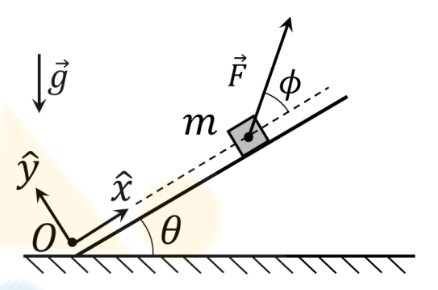
\includegraphics[scale=0.5]{figures/forca_minima.png}
\end{figure}

\subsection*{1) Equilíbrio de forças}

Projetando as forças ao longo dos eixos $\hat{x}$ (paralelo à rampa, apontando para cima) e $\hat{y}$ (normal ao plano):

\begin{equation}\label{eq:fx}
F\cos\varphi - mg\sin\theta - \mu N = 0
\end{equation}

\begin{equation}\label{eq:fy}
N - mg\cos\theta + F\sin\varphi = 0
\;\;\;\Rightarrow\;\;\;
N = mg\cos\theta - F\sin\varphi
\end{equation}

Substituindo \eqref{eq:fy} em \eqref{eq:fx}, obtemos:

\begin{equation}\label{eq:equil}
F\cos\varphi = mg\sin\theta + \mu\bigl(mg\cos\theta - F\sin\varphi\bigr).
\end{equation}

\subsection*{2) Expressão para a força aplicada}

Da equação \eqref{eq:equil}, resulta:

\begin{equation}\label{eq:fphi}
F(\varphi) = \frac{mg(\sin\theta + \mu\cos\theta)}{\cos\varphi + \mu\sin\varphi}.
\end{equation}

\subsection*{3) Maximização do denominador via Cauchy--Schwarz}

O denominador pode ser escrito como produto escalar:
\[
\cos\varphi + \mu\sin\varphi = (\cos\varphi,\;\sin\varphi)\cdot(1,\;\mu).
\]

Pela \colorbox{yellow!30}{desigualdade de Cauchy--Schwarz}:
\begin{equation}\label{eq:cauchy}
\boxed{
\cos\varphi + \mu\sin\varphi \le \sqrt{1+\mu^2}.
}
\end{equation}

A igualdade em \eqref{eq:cauchy} ocorre quando
\begin{equation}\label{eq:tanphi}
\tan\varphi^\star = \mu,
\end{equation}
isto é,
\[
\cos\varphi^\star = \frac{1}{\sqrt{1+\mu^2}},\qquad
\sin\varphi^\star = \frac{\mu}{\sqrt{1+\mu^2}}.
\]

\subsection*{4) Força mínima}

Substituindo o valor máximo do denominador \eqref{eq:cauchy} em \eqref{eq:fphi}, temos:

\begin{equation}\label{eq:fmin}
F_{\min} = \frac{mg(\sin\theta + \mu\cos\theta)}{\sqrt{1+\mu^2}}.
\end{equation}

Portanto, a força mínima aplicada que coloca o bloco na iminência de subir a rampa é dada por \eqref{eq:fmin}, atingida quando \eqref{eq:tanphi} vale.


\textbf{Alternativa correta:} \textbf{D}.
\end{flushleft}

\newpage

\noindent\rule{\linewidth}{0.6pt}\\

\begin{flushleft}
\subsection{Quest\~ao 42 — Cilindro com atrito}

Uma prancha de madeira, com comprimento $L = 1{,}0\ \text{m}$ e massa $m = 0{,}4\ \text{kg}$, 
possui um cilindro maciço e homogêneo de aço, com massa $M = 0{,}6\ \text{kg}$, 
localizado na extremidade direita da prancha. 
O sistema está em repouso sobre um plano horizontal liso. 
Uma força constante $\vec{F} = (20\ \text{N})\,\hat{x}$ é aplicada à prancha, 
fazendo com que os objetos comecem a se mover acelerados. 
O cilindro rola suavemente, sem escorregar, sobre a prancha, devido à presença de atrito entre eles. 
Desprezando o atrito entre a prancha e a superfície horizontal, bem como qualquer força de resistência do ar, 
determine o intervalo de tempo, em segundos, que o cilindro levará para cair da prancha, ou seja, 
para atingir a extremidade oposta e deixar de estar em contato com ela. 

\begin{figure}[!h]
  \centering
  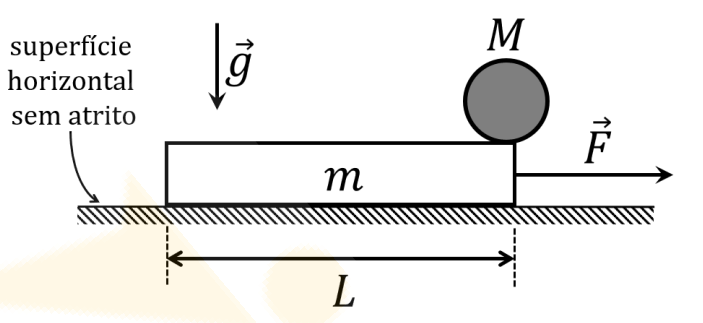
\includegraphics[scale=0.5]{figures/q42.png}
\end{figure}

\begin{itemize}
\item[(A)] 0,1 s
\item[(B)] 0,2 s
\item[(C)] 0,3 s
\item[(D)] 0,4 s
\item[(E)] 0,5 s
\end{itemize}

\subsection*{1) Definição das variáveis e forças}

Seja $a_p$ a aceleração da prancha (para a direita) e $a_c$ a aceleração do centro do cilindro (para a direita),
ambas medidas no referencial inercial do solo. Seja $f$ a força de atrito horizontal exercida pela prancha sobre o cilindro
(no ponto de contato). Pela ação e reação, a prancha sofre $-f$ da parte do cilindro.

Para o \colorbox{yellow!30}{cilindro maciço homogêneo, momento de inércia em relação ao centro:}
\begin{equation}\label{eq:I}
\boxed{
I=\frac{1}{2}MR^{2}.
}
\end{equation}

Não precisamos do valor de $R$ explicitamente, apenas das relações de rotação/translação.

\subsection*{2) Equações de movimento}

Equilíbrio (segunda lei) para a prancha (força total horizontal):
\begin{equation}\label{eq:plank}
F - f = m a_p .
\end{equation}

Equação de translação para o cilindro:
\begin{equation}\label{eq:cyl_trans}
f = M a_c .
\end{equation}

Equação de rotação para o cilindro (torque causado por $f$):
\begin{equation}\label{eq:cyl_rot}
fR = I \alpha = \left(\frac{1}{2}MR^{2}\right)\alpha.
\end{equation}

\textbf{\textcolor{red}{Condição de rolamento sem escorregar entre cilindro e prancha:
a velocidade do ponto de contato do cilindro iguala a velocidade da prancha.}} Em termos das acelerações:
\begin{equation}\label{eq:constraint}
a_c - a_p = -R\alpha.
\end{equation}

(A escolha do sinal garante consistência: se a prancha acelera mais que o cilindro, o contato induz uma rotação que satisfaz \eqref{eq:constraint}.)

\subsection*{3) Eliminação das incógnitas}

Da \eqref{eq:cyl_rot} e de \eqref{eq:constraint} obtemos:
\[
fR = \tfrac{1}{2}MR^{2}\alpha \quad\Rightarrow\quad f = \tfrac{1}{2}M R \alpha.
\]
Usando \eqref{eq:constraint} $\alpha = -(a_c - a_p)/R$, resulta
\begin{equation}\label{eq:f_from_rot}
f = -\tfrac{1}{2}M (a_c - a_p).
\end{equation}

Por outro lado, pela translação do cilindro \eqref{eq:cyl_trans}:
\begin{equation}\label{eq:f_from_trans}
f = M a_c.
\end{equation}

Igualando \eqref{eq:f_from_rot} e \eqref{eq:f_from_trans}:
\[
M a_c = -\tfrac{1}{2}M (a_c - a_p).
\]
Dividindo por $M$ e rearranjando:
\[
a_c = -\tfrac{1}{2}a_c + \tfrac{1}{2}a_p
\quad\Rightarrow\quad
\tfrac{3}{2}a_c = \tfrac{1}{2}a_p
\quad\Rightarrow\quad
a_c = \tfrac{1}{3} a_p. \label{eq:ac_ap}
\]

Substituindo \eqref{eq:ac_ap} em \eqref{eq:plank} e usando \eqref{eq:cyl_trans} ($f=M a_c$):
\[
F - M a_c = m a_p.
\]
Como $a_c = a_p/3$, obtemos
\[
F - M\frac{a_p}{3} = m a_p
\quad\Rightarrow\quad
F = a_p\!\left(m + \frac{M}{3}\right).
\]
Logo a aceleração da prancha:
\begin{equation}\label{eq:ap}
a_p = \frac{F}{\,m + \dfrac{M}{3}\,} = \frac{3F}{3m+M}.
\end{equation}
E, pela \eqref{eq:ac_ap},
\begin{equation}\label{eq:ac}
a_c = \frac{a_p}{3} = \frac{F}{3m+M}.
\end{equation}

\subsection*{4) Aceleração relativa e tempo até cair}

A aceleração relativa entre prancha e cilindro (aceleração com que a prancha “afasta-se” do cilindro) é
\[
a_{\text{rel}} = a_p - a_c = a_p - \frac{a_p}{3} = \frac{2}{3}a_p.
\]
Usando \eqref{eq:ap}:
\begin{equation}\label{eq:arel}
a_{\text{rel}} = \frac{2}{3}\cdot\frac{3F}{3m+M} = \frac{2F}{3m+M}.
\end{equation}

Inicialmente a velocidade relativa é zero (sistema parte do repouso). A distância relativa a percorrer para que
o cilindro passe da extremidade direita até a esquerda da prancha é $L$. Para movimento uniformemente acelerado,
o tempo $t$ satisfaz $L = \tfrac{1}{2} a_{\text{rel}} t^{2}$, portanto
\begin{equation}\label{eq:time_general}
t = \sqrt{\frac{2L}{a_{\text{rel}}}} = \sqrt{\frac{2L(3m+M)}{2F}} = \sqrt{\frac{(3m+M)\,L}{F}}.
\end{equation}

\subsection*{5) Substituição numérica}

Dados: $m=0{,}4\ \mathrm{kg}$, $M=0{,}6\ \mathrm{kg}$, $L=1{,}0\ \mathrm{m}$, $F=20\ \mathrm{N}$.

Calcule $3m+M$:
\[
3m+M = 3(0{,}4)+0{,}6 = 1{,}2+0{,}6 = 1{,}8\ \mathrm{kg}.
\]

Substituindo em \eqref{eq:time_general}:
\[
t = \sqrt{\frac{(3m+M) L}{F}}
= \sqrt{\frac{1{,}8\times 1{,}0}{20}}
= \sqrt{\frac{1{,}8}{20}}
= \sqrt{0{,}09}
= 0{,}30\ \mathrm{s}.
\]

\bigskip
\noindent\textbf{Resposta:} $t = 0{,}3\ \mathrm{s}$. (Alternativa \textbf{C}.)


\end{flushleft}

\noindent\rule{\linewidth}{0.4pt}\\

\begin{flushleft}
\subsection{Quest\~ao 43 - Trabalho de uma força de resistência}
\noindent
Um projétil de massa $m$ é lançado verticalmente para cima a partir da posição $z=0$ com velocidade inicial 
$\vec{v} = v_0 \hat{z}$ $(v_0>0)$ no instante $t=0$. Além da força gravitacional, atua sobre ele uma força de 
resistência do ar proporcional à velocidade: $\vec{F} = - \beta m \vec{v}$, onde $\beta>0$ é o parâmetro de amortecimento. 
A aceleração da gravidade é $\vec{g} = - g \hat{z}$. Determine o trabalho realizado pela força de resistência desde o lançamento até a altura máxima.

\vspace{0.5cm}

\textcolor{red}{\textbf{Solução:}}\\

A força de resistência é:
\[
\vec{F}_r = - \beta m \vec{v} = - \beta m v \hat{z}.
\]

O trabalho realizado pela força de resistência até a altura máxima é:
\[
W_r = \int_{0}^{z_\text{max}} \vec{F}_r \cdot d\vec{z} = - \beta m \int_0^{z_\text{max}} v \, dz.
\]

A \colorbox{red!20}{equação do movimento é}:
\[
m \frac{dv}{dt} = - mg - \beta m v \quad \Rightarrow \quad \boxed{\frac{dv}{dt} + \beta v = - g.}
\]

Solução da equação diferencial:

\[
\frac{dv}{dt} + \beta v = - g \Rightarrow \frac{dv}{dt} = - g - \beta v 
\]

\[
\frac{dv}{g+ \beta v} = - dt
\]

\[
\int \frac{dv}{g+ \beta v} = - \int dt
\]

\[
\frac{ln \left( g+ \beta v \right)}{\beta} = - t + C
\]

Usando as \colorbox{green!30}{condi\c{c}\~oes de contorno do problema (quando $t=0$ e $v=v_{o}$)}:

\[C = \frac{ln \left( g+ \beta v_0 \right)}{\beta}\]

\[
\frac{ln \left( g+ \beta v \right)}{\beta} = - t + \frac{ln \left( g+ \beta v_0 \right)}{\beta}
\]

\[
\frac{ln \left( g+ \beta v \right)}{\beta} - \frac{ln \left( g+ \beta v_0 \right)}{\beta} = - t
\]

\[
ln \left( g+ \beta v \right) - ln \left( g+ \beta v_0 \right) = - \beta t
\]

\[
ln \left[\frac{\left( g+ \beta v \right)}{ \left( g+ \beta v_0 \right)}\right] = - \beta t
\]

\[
\frac{\left( g+ \beta v \right)}{ \left( g+ \beta v_0 \right)} = e^{- \beta t}
\]

\[
\left( g+ \beta v \right)= \left( g+ \beta v_0 \right) e^{- \beta t}
\]

\[
\beta v = \left( g+ \beta v_0 \right) e^{- \beta t} - g
\]

\[
\boxed{
v(t) = \left(v_0 + \frac{g}{\beta}\right) e^{-\beta t} - \frac{g}{\beta}.
}
\]

\colorbox{green!30}{Altura máxima ocorre em $t_\text{max}$ tal que $v(t_\text{max}) = 0$}:
\[
0 = \left(v_0 + \frac{g}{\beta}\right) e^{-\beta t_\text{max}} - \frac{g}{\beta} 
\quad \Rightarrow \quad 
e^{-\beta t_\text{max}} = \frac{g/\beta}{v_0 + g/\beta} 
\quad \Rightarrow \quad \boxed{t_\text{max} = \frac{1}{\beta} \ln \left( 1 + \frac{\beta v_0}{g} \right).}
\]

O trabalho da força de resistência:
\[
W_r = - \beta m \int_0^{t_\text{max}} v^2(t) \, dt
= - \beta m \int_0^{t_\text{max}} \left[ \left(v_0 + \frac{g}{\beta}\right) e^{-\beta t} - \frac{g}{\beta} \right]^2 dt.
\]

\[
W_r = - \beta m \int_0^{t_\text{max}} \left[ \left(v_0 + \frac{g}{\beta}\right) e^{-\beta t} - \frac{g}{\beta} \right]^2 dt
\]

\[
\begin{aligned}
W_r &= - \beta m \int_0^{t_\text{max}} \Bigg[ 
\left(v_0 + \frac{g}{\beta}\right)^2 e^{-2\beta t} 
- 2 \left(v_0 + \frac{g}{\beta}\right) \frac{g}{\beta} e^{-\beta t} 
+ \left(\frac{g}{\beta}\right)^2 
\Bigg] dt \\
&= - \beta m \Bigg[ 
\left(v_0 + \frac{g}{\beta}\right)^2 \textcolor{red}{\int_0^{t_\text{max}} e^{-2\beta t} dt} 
- 2 \left(v_0 + \frac{g}{\beta}\right) \frac{g}{\beta} \textcolor{orange!90}{\int_0^{t_\text{max}} e^{-\beta t} dt }
+ \left(\frac{g}{\beta}\right)^2 \textcolor{blue}{\int_0^{t_\text{max}} dt}
\Bigg]
\end{aligned}
\]

\[
\begin{aligned}
\textcolor{red}{\int_0^{t_\text{max}} e^{-2\beta t} dt} &= \frac{1 - e^{-2 \beta t_\text{max}}}{2\beta}, \\
\textcolor{orange!90}{\int_0^{t_\text{max}} e^{-\beta t} dt } &= \frac{1 - e^{-\beta t_\text{max}}}{\beta}, \\
\textcolor{blue}{\int_0^{t_\text{max}} dt} & = t_\text{max}.
\end{aligned}
\]

Integrando e substituindo \(t_\text{max}\) e \(e^{-\beta t_\text{max}}\):

\[
t_\text{max} = \frac{1}{\beta} \ln \left( 1 + \frac{\beta v_0}{g} \right)
\]

\[
1 - e^{-2\beta t_\text{max}} = 1 - e^{-2\beta \left(\frac{1}{\beta} \ln \left( 1 + \frac{\beta v_0}{g} \right)\right)}
\]

\[
1 - e^{-2\beta t_\text{max}} = 1 - e^{-\ln \left( 1 + \frac{\beta v_0}{g} \right)^2}
\]

\[
1 - e^{-2\beta t_\text{max}} = 1 - \left( 1 + \frac{\beta v_0}{g} \right)^{-2}
\]

\[
1 - e^{-2\beta t_\text{max}} = 1 - \frac{1}{\left( 1 + \frac{\beta v_0}{g} \right)^{2}}
\]

\[
1 - e^{-2\beta t_\text{max}} = \frac{\left( 1 + \frac{\beta v_0}{g} \right)^{2} -1}{\left( 1 + \frac{\beta v_0}{g} \right)^{2}}
\]

\[
1 - e^{-2\beta t_\text{max}} = \frac{1 + \frac{2\beta v_0}{g} + \frac{\beta^2 v_0^2}{g^2} - 1}{\left( 1 + \frac{\beta v_0}{g} \right)^{2}}
\]

\[
\boxed{
1 - e^{-2\beta t_\text{max}} = \frac{\frac{2\beta v_0}{g} + \frac{\beta^2 v_0^2}{g^2}}{\left( 1 + \frac{\beta v_0}{g} \right)^{2}}
}
\]

\[
\boxed{
\begin{aligned}
\textcolor{red}{\int_0^{t_\text{max}} e^{-2\beta t} dt} &= \frac{1 - e^{-2 \beta t_\text{max}}}{2\beta} =  \frac{1}{2\beta} \frac{\left[\frac{2\beta v_0}{g} + \frac{\beta^2 v_0^2}{g^2} \right]}{\left(\frac{\beta}{g}\right)^2 \left( \frac{g}{\beta} + v_0 \right)^{2}}\\
\end{aligned}
}
\]

\[
\boxed{
\begin{aligned}
\textcolor{red}{\int_0^{t_\text{max}} e^{-2\beta t} dt} &= \frac{g^2}{2 \beta^3} \frac{\left[\frac{2\beta v_0}{g} + \frac{\beta^2 v_0^2}{g^2} \right]}{\left( v_0 + \frac{g}{\beta} \right)^{2}}. \quad \checkmark
\end{aligned}
}
\]

\[
1 - e^{-\beta t_\text{max}} = 1 - e^{-\beta \left(\frac{1}{\beta} \ln \left( 1 + \frac{\beta v_0}{g} \right)\right)}
\]

\[
1 - e^{-\beta t_\text{max}} = 1 - e^{\ln \left( 1 + \frac{\beta v_0}{g} \right)^{-1}}
\]

\[
1 - e^{-\beta t_\text{max}} = 1 - \left( 1 + \frac{\beta v_0}{g} \right)^{-1}
\]

\[
1 - e^{-\beta t_\text{max}} = 1 - \frac{1}{\left( 1 + \frac{\beta v_0}{g} \right)}
\]

\[
1 - e^{-\beta t_\text{max}} = \frac{\left( 1 + \frac{\beta v_0}{g} \right) - 1}{\left( 1 + \frac{\beta v_0}{g} \right)}
\]

\[
1 - e^{-\beta t_\text{max}} = \frac{\left(\frac{\beta v_0}{g} \right)}{\left( 1 + \frac{\beta v_0}{g} \right)}
\]

\[
1 - e^{-\beta t_\text{max}} = \frac{\left(\frac{\beta v_0}{g} \right)}{\left( 1 + \frac{\beta v_0}{g} \right)} = \frac{\left(\frac{\beta v_0}{g} \right)}{\frac{\beta}{g}\left( v_0 + \frac{g}{\beta} \right)} = \frac{v_0}{\left( v_0 + \frac{g}{\beta} \right)}
\]

\[
\begin{aligned}
\textcolor{orange!90}{\int_0^{t_\text{max}} e^{-\beta t} dt } &= \frac{1 - e^{-\beta t_\text{max}}}{\beta} = \frac{\frac{v_0}{\left( v_0 + \frac{g}{\beta} \right)}}{\beta} = \frac{v_0}{\beta\left( v_0 + \frac{g}{\beta} \right)} \\
\end{aligned}
\]

\[
\begin{aligned}
\textcolor{orange!90}{\int_0^{t_\text{max}} e^{-\beta t} dt } &= \frac{v_0}{\beta\left( v_0 + \frac{g}{\beta} \right)}. \quad \checkmark \\
\end{aligned}
\]


\[
\begin{aligned}
W_r &= - \beta m \Bigg[ 
\cancel{\left(v_0 + \frac{g}{\beta}\right)^2} \left[\frac{g^2}{2 \beta^3 } \frac{\left[\frac{2\beta v_0}{g} + \frac{\beta^2 v_0^2}{g^2} \right]}{\cancel{\left( v_0 + \frac{\beta}{g} \right)^{2}}}\right]
- 2 \cancel{\left(v_0 + \frac{g}{\beta}\right)}\frac{g}{\beta} \frac{v_0}{\beta\cancel{\left( v_0 + \frac{g}{\beta} \right)}} 
+ \left(\frac{g^2}{\beta^3}\right)\ln \left( 1 + \frac{\beta v_0}{g} \right)
\Bigg]
\end{aligned}
\]

\[
\begin{aligned}
W_r &= - \beta m \Bigg[ 
\frac{g^2 \left[\frac{2\beta v_0}{g} + \frac{\beta^2 v_0^2}{g^2} \right]}{2 \beta^3}
- 2 g\frac{v_0}{\beta} 
+ \left(\frac{g^2}{\beta^3}\right)\ln \left( 1 + \frac{\beta v_0}{g} \right)
\Bigg]
\end{aligned}
\]

\[
\begin{aligned}
W_r &= - \Bigg[ 
\frac{m g^2}{2 \beta^2} \left[\frac{2\beta v_0}{g} + \frac{\beta^2 v_0^2}{g^2} \right]
- 2 mg\frac{v_0}{\beta} 
+ \left(\frac{m g^2}{\beta^2}\right)\ln \left( 1 + \frac{\beta v_0}{g} \right)
\Bigg]
\end{aligned}
\]

\[
\begin{aligned}
W_r &= - \Bigg[ 
\frac{m g v_0 }{\beta}  + \frac{m v_0^2}{2}
- 2 mg\frac{v_0}{\beta} 
+ \left(\frac{m g^2}{\beta^2}\right)\ln \left( 1 + \frac{\beta v_0}{g} \right)
\Bigg]
\end{aligned}
\]

\[
\begin{aligned}
W_r &= 
- \frac{m g v_0 }{\beta} - \frac{m v_0^2}{2}
+ \frac{2 mg v_0}{\beta} 
- \left(\frac{m g^2}{\beta^2}\right)\ln \left( 1 + \frac{\beta v_0}{g} \right)
\end{aligned}
\]

\[
\begin{aligned}
W_r &= 
\frac{m g v_0 }{\beta}
- \left(\frac{m g^2}{\beta^2}\right)\ln \left( 1 + \frac{\beta v_0}{g} \right) - \frac{m v_0^2}{2}
\end{aligned}
\]

\[
\boxed{
\begin{aligned}
W_r &=  \frac{m g v_0 }{\beta} \Bigg[1 - \left(\frac{m g^2}{\beta^2}\right)\ln \left( 1 + \frac{\beta v_0}{g} \right) \Bigg] - \frac{m v_0^2}{2}
\end{aligned}
}
\quad \blacksquare
\]


\end{flushleft}


\begin{flushleft}

\subsection{Quest\~ao 44 - P\^endulo F\'isico}
Um p\^endulo f\'isico constitu\'{\i}do por uma placa fina e homog\^enea em forma de um setor circular de raio $R$ e \^angulo 
central $\alpha$, est\'a suspenso verticalmente no centro $O$ do disco de origem. O p\^endulo \'{e} deslocado por um \^angulo 
$\theta$ em rela\c{c}\~ao \`a vertical e, em seguida, abandonado a partir do repouso para oscilar. A acelera\c{c}\~ao local 
da gravidade \'e $g$ e poss\'iveis atritos s\~ao desprez\'iveis. Assinale a alternativa que apresenta a express\~ao correta 
para a frequ\^encia angular $\omega$ de pequenas oscila\c{c}\~oes do p\^endulo f\'isico.

\begin{figure}[!h]
  \centering
  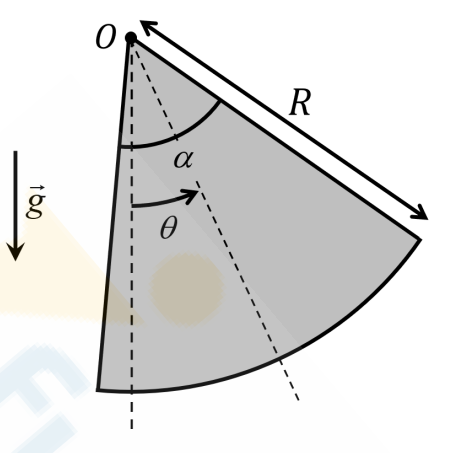
\includegraphics[scale=0.5]{figures/pendulo_fisico.png}
\end{figure}


\begin{itemize}
\item[(A)] $\displaystyle \omega=\sqrt{\frac{4g}{3R}}$
\item[(B)] $\displaystyle \omega=\sqrt{\frac{8g\cos(\alpha)}{3R\,\alpha}}$
\item[(C)] $\displaystyle \omega=\sqrt{\frac{8g\sin(\alpha/2)}{3R\,\alpha}}$
\item[(D)] $\displaystyle \omega=\sqrt{\frac{4g\sin(\alpha)}{3R\,\alpha}}$
\item[(E)] $\displaystyle \omega=\sqrt{\frac{4g\cos(\alpha/2)}{3R\,\alpha}}$
\end{itemize}

\vspace{0.5cm}

\textcolor{red}{\textbf{Solução:}}\\

Para \colorbox{yellow!30}{pequenas oscila\c{c}\~oes linearizamos $\sin\theta\approx\theta$ e usamos a equa\c{c}\~ao do p\^endulo f\'isico:}
\[
I_O\,\ddot\theta + m g h\,\theta = 0,
\]

\[
\,\ddot\theta + \frac{m g h}{I_O}\,\theta = 0,
\]

\[
\,\ddot\theta + \omega^{2}\,\theta = 0,
\]


onde $I_O$ \'e o momento de in\'ercia em rela\c{c}\~ao ao ponto de suspens\~ao $O$ (eixo perpendicular ao plano) e $h$ \'e a dist\^ancia 
do centro de massa ao ponto $O$.

\textbf{1) Massa e momento de in\'ercia:}\\
Para uma placa homog\^enea em forma de setor, a densidade superficial $\sigma$ satisfaz
\[
m=\sigma\cdot\text{área}=\sigma\left(\tfrac{1}{2}\alpha R^2\right).
\]
O momento de in\'ercia em rela\c{c}\~ao a $O$ (eixo perpendicular ao plano) é
\[
I_O=\sigma\int_{0}^{\alpha}\int_{0}^{R} r^2\;r\,dr\,d\phi
=\sigma\frac{\alpha R^4}{4}.
\]
Substituindo $\sigma = \dfrac{2m}{\alpha R^2}$ obtemos
\[
I_O=\frac{2m}{\alpha R^2}\cdot\frac{\alpha R^4}{4}=\frac{mR^2}{2}.
\]

\textbf{2) Centro de massa (distância radial $h$ a partir de $O$):}\\
O centro de massa de um setor circular encontra-se sobre a bissetriz e sua distância ao centro é
\[
\boxed{
h=r_{CM}=\frac{4R\sin(\alpha/2)}{3\alpha}.
}
\]

\textbf{3) Frequência angular:}\\
\[
\omega=\sqrt{\frac{m g h}{I_O}}
=\sqrt{\frac{m g \,\dfrac{4R\sin(\alpha/2)}{3\alpha}}{\dfrac{mR^2}{2}}}
=\sqrt{\frac{8g\sin(\alpha/2)}{3R\,\alpha}}.
\]

Portanto, a alternativa correta é \(\colorbox{green!50}{\textbf{(C)}}\).

\end{flushleft}


\begin{flushleft}
\subsection{Quest\~ao 45 - Colis\~ao Unidimensional inel\'astica}

Considere uma part\'icula de massa $m$, que se move com velocidade $v_0$, e realiza uma colis\~ao unidimensional inel\'astica com outra part\'icula de massa $M$, inicialmente em repouso. O coeficiente de restitui\c{c}\~ao do material constituinte das part\'iculas \'e denotado por $\varepsilon$. Considerando que a raz\~ao das massas das part\'iculas \'e $M/m=\lambda$, analise as assertivas abaixo:

I. A velocidade da part\'icula de massa $m$ ap\'os a colis\~ao \'e $v=v_0(1-\varepsilon\lambda)/(1+\lambda)$.\\
II. A velocidade da part\'icula de massa $M$ ap\'os a colis\~ao \'e $V=v_0(1+\varepsilon)/(1+\lambda)$.\\
III. A raz\~ao entre a energia cin\'etica adquirida pela part\'icula de massa $M$ e a energia cin\'etica inicial da part\'icula de massa $m$ \'e $\lambda(\varepsilon+1)/(\lambda+1)$.

Quais est\~ao corretas?

\begin{itemize}
\item[(A)] Apenas I.
\item[(B)] Apenas II.
\item[(C)] Apenas III.
\item[(D)] Apenas I e II.
\item[(E)] I, II e III.
\end{itemize}

\vspace{0.5cm}

\textcolor{red}{\textbf{Solução:}}\\

Pela conserva\c{c}\~ao do momento e defini\c{c}\~ao do coeficiente de restitui\c{c}\~ao:
\[
m v_0 = m v + M V,
\qquad
V - v = \varepsilon (v_0-0)=\varepsilon v_0.
\]
Da segunda equa\c{c}\~ao temos $V=v+\varepsilon v_0$. Substituindo na conserva\c{c}\~ao do momento:
\[
m v_0 = m v + M(v+\varepsilon v_0)=(m+M)v + M\varepsilon v_0.
\]
Isolando $v$:
\[
(m+M)v = v_0(m - M\varepsilon)
\quad\Rightarrow\quad
v = v_0\frac{m - M\varepsilon}{m+M}
= v_0\frac{1-\lambda\varepsilon}{1+\lambda},
\]
o que confirma a assertiva \textbf{I}.

Agora $V=v+\varepsilon v_0$:
\[
V=v_0\frac{1-\lambda\varepsilon}{1+\lambda}+\varepsilon v_0
= v_0\frac{1-\lambda\varepsilon+\varepsilon(1+\lambda)}{1+\lambda}
= v_0\frac{1+\varepsilon}{1+\lambda},
\]
confirmando a assertiva \textbf{II}.

Para a assertiva \textbf{III}, calculemos a raz\~ao das energias:
\[
\frac{K_M}{K_{m,\,\text{inicial}}}
=\frac{\tfrac{1}{2}M V^2}{\tfrac{1}{2}m v_0^2}
=\frac{M}{m}\left(\frac{V}{v_0}\right)^2
=\lambda\left(\frac{1+\varepsilon}{1+\lambda}\right)^2
=\frac{\lambda(1+\varepsilon)^2}{(1+\lambda)^2},
\]
que \textbf{não} coincide com $\dfrac{\lambda(1+\varepsilon)}{1+\lambda}$ (a dada na III). Portanto a assertiva \textbf{III} é falsa.

Assim, est\~ao corretas apenas I e II.

A resposta correta é alternativa \colorbox{green!50}{\textbf{(D)}}.

\end{flushleft}

\begin{flushleft}
\subsection{Quest\~ao 47 - Oscila\c{c}\~oes acopladas}

Dois blocos (1 e 2) de massas iguais a  $m = 0,5\,\text{kg}$ são conectados a três molas que
estão posicionadas entre duas paredes, conforme ilustrado na figura abaixo. A constante elástica das
duas molas externas é $k = 2,0\,\text{N/m}$, e a constante elástica da mola do meio $k_0 = 8,0\,\text{N/m}$. As molas
têm massa desprezível e satisfazem à lei de Hooke. Sabe-se também que quando os blocos se
encontram simultaneamente em suas respectivas posições de equilíbrio, as molas não apresentam
qualquer deformação. Considere que $x_1(t)$ e $x_2(t)$ denotam os deslocamentos dos blocos da esquerda
e da direita, respectivamente, em relação às suas posições de equilíbrio. No instante inicial $t$ = 0,
ambos os blocos 1 e 2 são soltos a partir do repouso nas posições $x_1(0)=10\,\text{cm}$ e $x_2(0)=0$,
respectivamente. Assinale a alternativa que representa a posição dos blocos como função do tempo
medido em unidades do sistema internacional.

\begin{figure}[!h]
  \centering
  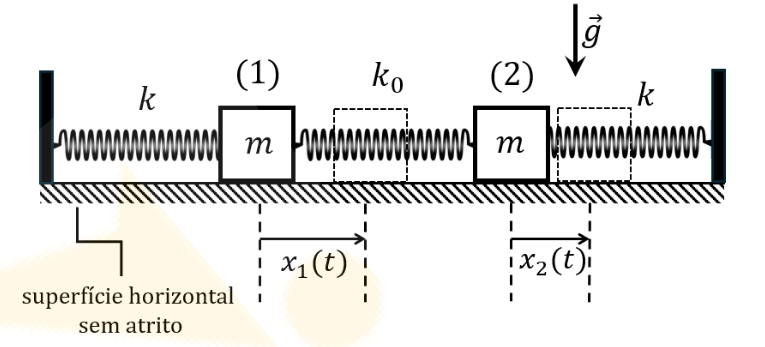
\includegraphics[scale=0.5]{figures/sistema-massa-mola.png}
\end{figure}

\begin{itemize}
\item[(A)] $x_1(t)=0,05[\cos(2t)+\cos(6t)]\,\text{m}, \;\; x_2(t)=0,05[\cos(2t)-\cos(6t)]\,\text{m}$
\item[(B)] $x_1(t)=0,05[\cos(2t)+\cos(4t)]\,\text{m}, \;\; x_2(t)=0,05[\cos(4t)-\cos(2t)]\,\text{m}$
\item[(C)] $x_1(t)=0,05\cos(3t)\cos(t)\,\text{m}, \;\; x_2(t)=0,05\sin(3t)\sin(t)\,\text{m}$
\item[(D)] $x_1(t)=0,10\cos(4t)\,\text{m}, \;\; x_2(t)=0,10\sin(2t)\,\text{m}$
\item[(E)] $x_1(t)=0,10\cos(2t)\,\text{m}, \;\; x_2(t)=0,10\sin(4t)\,\text{m}$
\end{itemize}

\vspace{0.5cm}

\textcolor{red}{\textbf{Solu\c{c}\~ao:}}\\[2mm]

1) \textbf{Equa\c{c}\~oes de movimento:}  
Para o bloco 1:
\[
m\ddot{x}_1 = -k x_1 - k_0(x_1 - x_2).
\]

Para o bloco 2:
\[
m\ddot{x}_2 = -k x_2 - k_0(x_2 - x_1).
\]

\[
\Rightarrow 
\begin{cases}
\ddot{x}_1 + \dfrac{k+k_0}{m}x_1 - \dfrac{k_0}{m}x_2 = 0, \\
\ddot{x}_2 + \dfrac{k+k_0}{m}x_2 - \dfrac{k_0}{m}x_1 = 0.
\end{cases}
\]

2) \textbf{Matriz do sistema:}  
\[
\begin{bmatrix}
\ddot{x}_1 \\ \ddot{x}_2
\end{bmatrix}
= -\frac{1}{m}
\begin{bmatrix}
k+k_0 & -k_0 \\
-k_0 & k+k_0
\end{bmatrix}
\begin{bmatrix}
x_1 \\ x_2
\end{bmatrix}.
\]

Com $m=0,5$, $k=2$ e $k_0=8$:
\[
A=\frac{1}{0,5}
\begin{bmatrix}
10 & -8 \\ -8 & 10
\end{bmatrix}
=
\begin{bmatrix}
20 & -16 \\ -16 & 20
\end{bmatrix}.
\]

3) \textbf{Autovalores (modos normais):}  
\[
\det(A-\lambda I)=0 \;\;\Rightarrow\;\;
(20-\lambda)^2-(-16)^2=0,
\]
\[
(20-\lambda)^2-256=0,
\;\;\Rightarrow\;\;
20-\lambda=\pm 16.
\]
\[
\lambda_1=4, \quad \lambda_2=36.
\]

Logo, as frequ\^encias s\~ao:
\[
\omega_1=\sqrt{4}=2, \qquad \omega_2=\sqrt{36}=6.
\]

4) \textbf{Autovetores:}  
Para $\lambda_1=4$:  
\[
(20-4)x_1-16x_2=0 \;\;\Rightarrow\;\; x_1=x_2.
\]

Para $\lambda_2=36$:  
\[
(20-36)x_1-16x_2=0 \;\;\Rightarrow\;\; x_1=-x_2.
\]

\textbf{Modos normais:}
\[
\begin{cases}
\text{Modo 1 (freq. 2 rad/s): } x_1=x_2, \\
\text{Modo 2 (freq. 6 rad/s): } x_1=-x_2.
\end{cases}
\]

5) \textbf{Combina\c{c}\~ao linear:}  
Solu\c{c}\~ao geral:
\[
x_1(t)=A\cos(2t)+B\cos(6t), \quad
x_2(t)=A\cos(2t)-B\cos(6t).
\]

6) \textbf{Condi\c{c}\~oes iniciais:}  
No instante $t=0$:
\[
x_1(0)=A+B=0,10, \quad x_2(0)=A-B=0.
\]

\[
A=B=0,05.
\]

7) \textbf{Solu\c{c}\~ao final:}
\[
x_1(t)=0,05[\cos(2t)+\cos(6t)] \;\text{m}, \qquad
x_2(t)=0,05[\cos(2t)-\cos(6t)] \;\text{m}.
\]

\medskip

A resposta correta \'e a alternativa \colorbox{green!50}{\textbf{(A)}}.

\end{flushleft}


\section{Gravita\c{c}\~ao}

\begin{flushleft}
\subsection{Quest\~ao 46 - Balan\c{c}a de tor\c{c}\~ao de Cavendish}

No experimento de Henry Cavendish, de 1797, foi utilizada uma balan\c{c}a de tor\c{c}\~ao
para determinar o valor da constante gravitacional $G$ da lei da gravita\c{c}\~ao universal de Newton.
Considere uma balan\c{c}a de tor\c{c}\~ao composta por uma barra de massa desprez\'ivel e comprimento $L$,
suspensa horizontalmente pelo seu centro por um fio de tor\c{c}\~ao vertical. Duas pequenas esferas de
massa igual a $m$ est\~ao presas em cada extremidade da barra. No primeiro passo do experimento,
observa-se que, quando a barra \'e girada com um pequeno \^angulo, torcendo o fio, e depois solta, o
p\^endulo de tor\c{c}\~ao resultante sofre movimento harm\^onico simples com um per\'iodo $T$. Em seguida,
ap\'os o p\^endulo ser parado e estar em sua posi\c{c}\~ao de equil\'ibrio, um par de esferas grandes de massa
igual a $M$ s\~ao colocadas em lados opostos da barra, cada uma pr\'oxima a uma das massas $m$. Devido
\`a atra\c{c}\~ao gravitacional apenas entre cada par de massas, a barra \'e observada girando por um pequeno
\^angulo $\theta$ e depois parar nessa posi\c{c}\~ao, com cada massa $M$ a uma dist\^ancia $D$ da massa $m$
correspondente. Determine uma express\~ao para $G$ em termos das vari\'aveis dadas no problema.

\begin{figure}[!h]
  \centering
  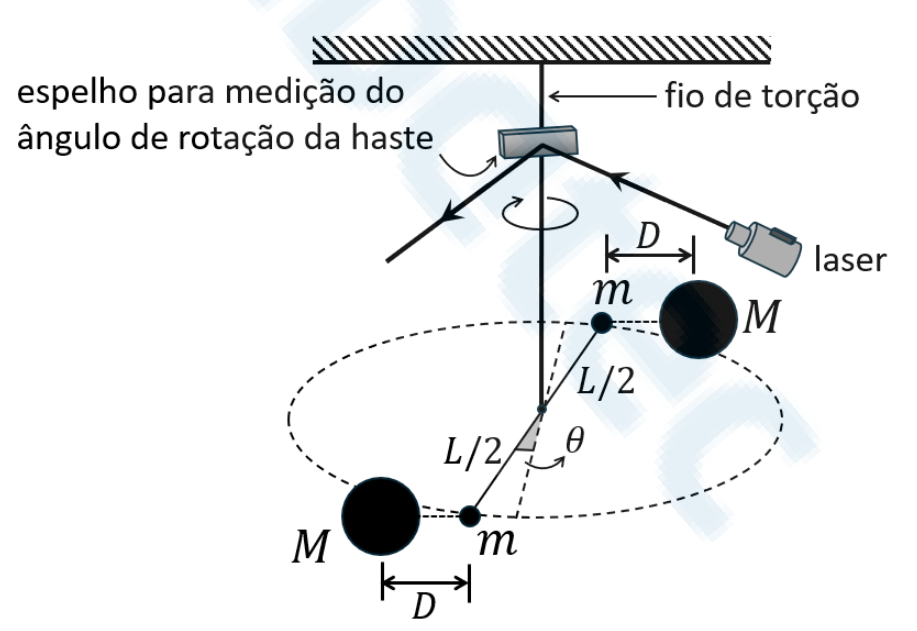
\includegraphics[scale=0.3]{figures/henry_cavendish.png}
\end{figure}

\begin{itemize}
\item[(A)] $\,G=\dfrac{\pi^2 D^2 L^2 \theta}{M T^2}$
\item[(B)] $\,G=\dfrac{2\pi^2 D^2 L \theta}{M T^2}$
\item[(C)] $\,G=\dfrac{4\pi^2 D^2 L^2 \theta}{M T^2}$
\item[(D)] $\,G=\dfrac{\pi^2 D^2 L \theta}{m T^2}$
\item[(E)] $\,G=\dfrac{\pi^2 D^2 L \theta}{4m T^2}$
\end{itemize}

\vspace{0.5cm}

\textcolor{red}{\textbf{Solu\c{c}\~ao:}}\\[2mm]

1) \textbf{\colorbox{yellow!30}{Constante de tor\c{c}\~ao via o per\'iodo.}} Para pequenas oscila\c{c}\~oes, o p\^endulo de tor\c{c}\~ao satisfaz
\[
T=2\pi\sqrt{\frac{I}{\kappa}}
\quad\Rightarrow\quad
\boxed{\kappa=\frac{4\pi^2 I}{T^2}}.
\]
A barra \'e desprez\'ivel e h\'a duas massas $m$ a $L/2$ do eixo, logo
\[
I=2\,m\left(\frac{L}{2}\right)^2=\frac{mL^2}{2}
\;\;\Rightarrow\;\;
\kappa=\frac{4\pi^2}{T^2}\,\frac{mL^2}{2}
=\frac{2\pi^2 m L^2}{T^2}.
\]

2)  \textbf{\colorbox{yellow!30}{Equil\'ibrio com as massas $M$.}} A for\c{c}a gravitacional entre $M$ e $m$ \'e
\[
F=\frac{G m M}{D^2}.
\]
Cada for\c{c}a produz um torque de m\'odulo $F\cdot (L/2)$ em torno do centro; s\~ao duas for\c{c}as sim\'etricas, portanto o torque gravitacional total vale
\[
\tau_g=2\,F\left(\frac{L}{2}\right)=F\,L.
\]
No novo equil\'ibrio, \colorbox{yellow!30}{o torque el\'astico do fio $\tau_{\kappa}=\kappa\,\theta$ (para pequeno $\theta$)} equilibra o torque gravitacional:
\[
\kappa\,\theta=F\,L=\frac{G m M}{D^2}\,L.
\]

3) \textbf{Isolando $G$.} Substituindo $\kappa$:
\[
\frac{2\pi^2 m L^2}{T^2}\,\theta=\frac{G m M}{D^2}\,L
\;\;\Rightarrow\;\;
\boxed{G=\frac{2\pi^2 D^2 L\,\theta}{M T^2}.}
\]

\medskip

A resposta correta \'e a alternativa \colorbox{green!50}{\textbf{(B)}}.

\end{flushleft}

\begin{flushleft}
\subsection{Questão 48 - Módulo da velocidade de um satélite orbitando a Terra}
Um satélite artificial orbita a Terra em uma trajetória elíptica sob efeito apenas da
força gravitacional. O satélite passa pelo perigeu $P$ (ponto mais próximo à Terra) com velocidade $\vec{v}_p$ e
pelo apogeu $A$ (ponto mais afastado da Terra) com velocidade $\vec{v}_a$. A velocidade do satélite em um
ponto $Y$, localizado na linha que passa pela Terra e perpendicular ao eixo maior da elipse, é denotada
por $\vec{v}$. É correto afirmar que o módulo da velocidade $v$ no ponto $Y$, em termos de $v_p$ e $v_a$ , é expresso
por:

\begin{figure}[!h]
  \centering
  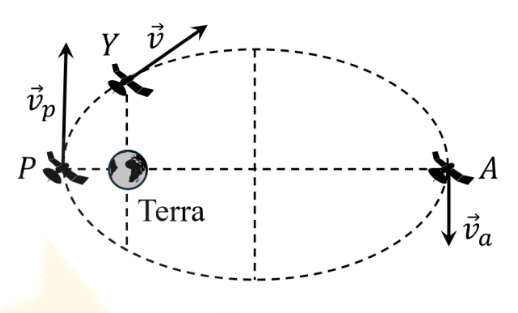
\includegraphics[scale=0.6]{figures/satelite.png}
\end{figure}

\begin{itemize}
\item[(A)] $v = \dfrac{v_a+v_p}{2}$
\item[(B)] $v = \dfrac{2v_av_p}{v_a+v_p}$
\item[(C)] $v = \sqrt{v_av_p}$
\item[(D)] $v = \sqrt{\dfrac{v_a^2+v_p^2}{2}}$
\item[(E)] $v = \sqrt{\dfrac{2v_a^2v_p^2}{v_a^2+v_p^2}}$
\end{itemize}

\vspace{0.5cm}

\textcolor{red}{\textbf{Solução:}}\\

Considerando a órbita elíptica com foco na Terra, usemos a equação de \emph{vis-viva} e a conservação do momento angular. Denotando por $\mu=GM$,

\[
v^2=\mu\!\left(\frac{2}{r}-\frac{1}{a}\right),
\]
onde $r$ é a distância ao foco (Terra) no ponto considerado e $a$ é o semieixo maior. Para o perigeu ($r_p$) e apogeu ($r_a$) temos
\begin{align}
v_p^2&=\mu\!\left(\frac{2}{r_p}-\frac{1}{a}\right),\label{vp}\\
v_a^2&=\mu\!\left(\frac{2}{r_a}-\frac{1}{a}\right).\label{va}
\end{align}

Subtraindo \eqref{va} de \eqref{vp} obtemos
\[
v_p^2-v_a^2=2\mu\!\left(\frac{1}{r_p}-\frac{1}{r_a}\right)
\quad\Rightarrow\quad
\mu=\frac{v_p^2-v_a^2}{2\left(\dfrac{1}{r_p}-\dfrac{1}{r_a}\right)}.
\]

O ponto $Y$ corresponde ao ângulo verdadeiro $\theta=\tfrac{\pi}{2}$, portanto
\[
r_Y=\frac{a(1-e^2)}{1+0}=a(1-e^2).
\]
Usando a relação entre os raios de perigeu/apogeu e $a$ (isto é, $r_p=a(1-e)$ e $r_a=a(1+e)$) obtemos
\[
\frac{1}{r_Y}=\frac{a}{r_pr_a}=\frac{r_p+r_a}{2r_pr_a}.
\]

Agora escrevemos a velocidade em $Y$ via vis-viva (usando a expressão em $r_p$ e eliminando $1/a$):
\[
v_Y^2=v_p^2+2\mu\!\left(\frac{1}{r_Y}-\frac{1}{r_p}\right).
\]
Substituindo $\mu$ e $\dfrac{1}{r_Y}-\dfrac{1}{r_p}=\dfrac{r_p-r_a}{2r_pr_a}$ temos
\[
v_Y^2
= v_p^2 + (v_p^2-v_a^2)\frac{r_pr_a}{r_a-r_p}\cdot\frac{r_p-r_a}{2r_pr_a}
= v_p^2 -\frac{1}{2}(v_p^2-v_a^2).
\]
Portanto
\[
v_Y^2=\frac{v_p^2+v_a^2}{2},
\]
e
\[
\boxed{\,v_Y=\sqrt{\dfrac{v_p^2+v_a^2}{2}}\,.}
\]

\textbf{Resposta:} alternativa \(\colorbox{green!50}{\textbf{D}}\).

\end{flushleft}

%%%%%%%%%%%%%%%%%%%%%%%%%%%%%%%%%%%%%%%%%%%%%%%%%%%%%%%%%%%%%%%%%%
\newpage 

\begin{flushleft}
\textbf{Problema.} Um pêndulo de massa $m_2$ e comprimento $L$ é solto do repouso na posição $A$, que faz um ângulo $\theta$ com a vertical. A corda passa por uma roldana ideal e traciona um bloco de massa $m_1$ sobre uma mesa horizontal. Ao o pêndulo atingir o ponto mais baixo $B$, qual deve ser o menor coeficiente de atrito estático $\mu_s$ entre $m_1$ e a mesa para que $m_1$ não deslize?

\vspace{0.4cm}
\textbf{Solução.}

\textit{1) Velocidade do pêndulo em $B$.} Pela conservação de energia entre $A$ e $B$:
\[
m_2 g L\,(1-\cos\theta)=\frac12 m_2 v_B^2
\;\;\Rightarrow\;\;
v_B^2=2gL\,(1-\cos\theta).
\]

\textit{2) Tração na corda em $B$.} No ponto mais baixo, as forças radiais no pêndulo dão
\[
T_B - m_2 g = m_2\frac{v_B^2}{L}
\;\;\Rightarrow\;\;
T_B = m_2\!\left(g+\frac{v_B^2}{L}\right)
     = m_2 g\bigl[1+2(1-\cos\theta)\bigr]
     = m_2 g\,(3-2\cos\theta).
\]

Como a roldana é ideal, a tração que puxa $m_1$ na horizontal é $T_B$.

\textit{3) Condição de não deslizamento de $m_1$.} Para $m_1$ permanecer em repouso,
a força de atrito estático máxima deve ser ao menos igual à tração:
\[
f_{s,\max}=\mu_s N=\mu_s m_1 g \;\ge\; T_B.
\]
Logo, o coeficiente mínimo é
\[
\boxed{\;\mu_{s,\min}=\frac{T_B}{m_1 g}
      =\frac{m_2}{m_1}\,\bigl(3-2\cos\theta\bigr)\; }.
\]

\textbf{Observação:} O ponto $B$ é o ponto mais baixo da trajetória, onde a tração é máxima; portanto, se $m_1$ não desliza em $B$, não deslizará em nenhuma outra posição.
\end{flushleft}




%%%%%%%% Bibliography 
% Os comandos para incluir as referências bibliográficas
%\printingbibliography

\end{document}
